\documentclass[aspectratio=169]{beamer}
% TODO cambiar a la de dalt
%\documentclass[aspectratio=169,handout]{beamer}
\usepackage{pgfpages}

%
% ============ APARTATS ============
% i) Definició del models SUM I MAX.
% ii) Computar la Best response és NP-hard en el dos models (SUM I MAX) 
%     (Theorem 1 i doneu tots els details que pugueu tan per MAX com per SUM)
%

% ============== TODO ===============
% - Network Creation Games:
%    + explicar PoS i PoA 
% - Model SUM: 
%    + diameter, etc
% - Model MAX:
%    + diameter, etc
% - k-MEDIAN
%    + explicar per sobre com sabem que es NP-hard
% - k-CENTER
%    + explicar per sobre com sabem que es NP-hard

%\setbeameroption{show only notes}
\setbeameroption{show notes on second screen}

\usepackage[catalan]{babel}
\usepackage[utf8]{inputenc}
\usepackage[T1]{fontenc}

\usepackage[style=english]{csquotes}

\usepackage[
backend=biber,
%style=apa,
%sorting=ynt
]{biblatex}
\addbibresource{biblio.bib}

\usetheme{Madrid}
\useinnertheme{rectangles}
\usefonttheme{professionalfonts}
\usecolortheme{crane}
\setbeamertemplate{blocks}[default]
\setbeamersize{text margin left=10mm,text margin right=10mm} 

\usepackage{times} 
\usepackage{booktabs}
\usepackage[scale=2]{ccicons}
\usepackage{xspace}
\usepackage{graphicx}
%\usepackage{enumitem}

\usepackage{amsmath}
\usepackage{tikz}

\DeclareMathOperator{\dist}{dist}
\DeclareMathOperator{\SUM}{SUM}
\DeclareMathOperator{\MAX}{MAX}

\newcommand{\kcenter}{\texorpdfstring{$k$}{k}-\textsc{center}\xspace}
\newcommand{\kmedian}{\texorpdfstring{$k$}{k}-\textsc{median}\xspace}

\setbeamercovered{transparent}

\definecolor{darkblue}{RGB}{4,9,73}

\title[Bounded Budget Network Creation Game]{Bounded Budget Network Creation Game}
\subtitle{}
\author{Grup 1}
\institute{UPC - AA}
\date{10 de juny de 2020}

\begin{document}

\begin{frame}
  \titlepage
  \note{HELLO}
  \note[item]{test}
\end{frame}

\begin{frame}{Index}
  \tableofcontents
\end{frame}

\section{Introducció}

\begin{frame}{Introducció}
    \setlength{\leftmargini}{10em}
    \begin{itemize}
        \itemsep=1em
        \item[\textbf{Article:}] Bounded Budget Network Creation Game
        \item[\textbf{Autors:}] Sayan Ehsani, Saber Shokat Fadaee, Mohammadamin Fazli, Abbas Mehrabian, Sina Sadeghian Sadeghabad, Mohammadali Safari and Morteza Saghafian
        \item[\textbf{Publicació:}] ACM Transaction on Algorithms, Vol. 11, No. 4, Article 34
        \item[\textbf{Data de publicació:}] Abril 2015
        \item[\textbf{DOI:}] 10.1145/2701615
    \end{itemize}
\end{frame}

\subsection{Network Creation Games}
\setbeamercovered{transparent}
\begin{frame}{Network Creation Games}
    %Un Network Creation Game és un joc que modela la creació d'una xarxa a través d'un graf.
    
    \onslide<1->{Un \emph{Network creation game} es centra en \textbf{modelar xarxes} de la vida real des del punt de vista de la \textbf{teoria de jocs}.}
    
    \vspace{1em}
    
    % nose
    
    % Selfish Network Creation focuses on modeling real world networks from a game-theoretic pointof view. 
    % One of the classic models by Fabrikant et al. [PODC’03] is the network creation game,where agents correspond 
    % to nodes in a network which buy incident edges for the price ofαperedge to minimize their total distance to all other nodes

\note{
 Hi ha moltes variants de jocs. La que expliquem aquí es la mes típica (la d classe).
 La que s estudia al article es un altre que no te $\alpha$
}
    
    \onslide<2->{\textbf{Cada node $u$ representa un jugador} i \textbf{cada jugador té una estratègia $S_u$}, representada per un conjunt d'arestes que el jugador
    crea, on cada aresta té cost de creació $\alpha$.}
    
    \vspace{1em}
    
    \onslide<3->{El vector d'estratègia $S = (S_1,...,S_n)$ conté l'estratègia de cada jugador i $G(S)$ és el graf no-dirigit resultant d'aplicar les estratègies.}
    
    \vspace{1em}
    
    \onslide<4->{\textbf{Objectiu} de cada node:
    \begin{itemize}
        \item Minimitzar la creació d'arestes
        \item Minimitzar la distància als altres nodes
    \end{itemize}}
    
\end{frame}

\begin{frame}{Network Creation Games}
    Cada node vol minimitzar la seva funció de cost, que definim com:
    \begin{equation*}
        c(u) = \alpha n_u + \sum_{v \in V(G)}\dist(u,v)
    \end{equation*}
    On $n_u = |S_u|$ i $G$ és el graf que representa la xarxa.
    
    \vspace{1.5em}
    
    Definim el \textbf{cost social} com la suma dels costos de tots els nodes:
    \begin{equation*}
        SC(S) = \alpha |E| + \sum_{u,v \in V(G)} \dist(u,v)
    \end{equation*}
\end{frame}

\begin{frame}{Network Creation Games}
    El \textbf{preu de l'anarquia} (\emph{PoA}) mesura la pèrdua d'eficiència deguda a l'actitud egoista dels jugadors. Es calcula:
    \begin{equation*}
        PoA = \frac{\max_{s \in S} SC(s)}{\min_{e \in E} SC(e)}
    \end{equation*}
    On $E \subseteq S$ és el conjunt amb totes les estratègies que són equilibris.
\end{frame}

\subsection{Bounded Budget Network Creation Game}
\begin{frame}{Bounded Budget Network Creation Game}
Definicions:
\begin{itemize}
    \item Donat un graf dirigit $G$, denotem el seu conjunt de vèrtexs com $V(G)$.
    \item $U(G)$ es un graf no-dirigit obtingut ignorant les direccions en $G$.
    \item Si $\overrightarrow{uv}, \overrightarrow{vu} \in G$ llavors $uv \in U(G)$ te multiplicitat $2$ i
        anomenem la parella $\{u, v\}$ \emph{brace}.
    \item $\dist(u, v)$ denota la distancia entre $u$ i $v$ a $U(G)$.
    \item Si $u$ i $v$ estan en components connexos diferents de $U(G)$ llavors
        $\dist(u, v) = C_{inf} = n^2$.
    \item No tenim $\alpha$, és a dir, les arestes no tenen cost.
        
    \note{El motiu del valor de $C_{inf} = n^2$ s'explica més endavant a $\SUM$} 
    
\end{itemize}
\end{frame} 

\begin{frame}{Bounded Budget Network Creation Game}
    Denotem un \emph{Bounded budget network creation game} com:
    $$ (b_1, b_2, \dots , b_n)\text{-BG} $$
    
    On $b_1,b_2, \dots , b_n$ són enters no negatius que representen el pressupost de cada jugador ($n$ és el nombre de jugadors).
    
    \vspace{1em}
    
    Cada jugador $i$ té assignada una estratègia $S_i \subseteq \{1, 2, \dots , n\} \backslash \{i\}$ amb
    $|S_i| = b_i$.
    
    \vspace{1em}
    
    Podem construir un graf $G$ a partir del conjunt de totes les estratègies afegint un vèrtex $\overrightarrow{u_iv_j}$
    a $G$ si i només si $j \in S_i$. Anomenen a aquests grafs \emph{realitzadors} de
    $ (b_1, b_2, \dots , b_n)\text{-BG} $.
    
    \vspace{1em}
    
    Direm que un vèrtex està en la millor resposta (\emph{best response}) si no pot disminuir el seu
    cost mantenint fixes les estratègies de la resta de vèrtexs.
\end{frame}

\begin{frame}{Bounded Budget Network Creation Game}
    
    %\color{darkblue}
    %{\Large Exemple}
    %\color{black}
    %
    %\vspace{1em}
    
    \begin{center}
    $(2,2,1,0)-\text{BG}$ \qquad $S = (\{2,4\},\{1,4\},\{2\},\{\})$
    \end{center}

    \vspace{1em}

    \begin{columns}
        \begin{column}{0.5\textwidth}
        \centering
        \begin{figure}
        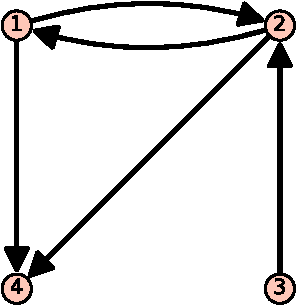
\includegraphics[scale=0.75]{digraph-crop}
        \end{figure}
        \vspace{-1em}
        {\large $G$}
        \end{column}
        
        \begin{column}{0.5\textwidth}
        \centering
        \begin{figure}
        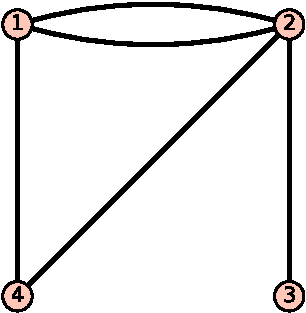
\includegraphics[scale=0.75]{u-crop}
        \end{figure}
        \vspace{-1em}
        {\large $U(G)$}
        \end{column}
    \end{columns}    
    
\end{frame}

% \begin{frame}{Bounded Budget Network Creation Game}
%     Per aquest joc
% \end{frame}

\section{Definició dels models}

\begin{frame}{Definició dels models}
    A l'article~\cite{ehsani_bounded_2015} es consideren 2 models de \emph{bounded budget network creation games}:
    
    \vspace{1.5em}
    
    \begin{itemize}
    \item $\SUM$
    \item $\MAX$
    \end{itemize}
    
    \vspace{3em}
    
    Els models difereixen en la definició de la funció de cost.
\end{frame}

\subsection{\texorpdfstring{$\SUM$}{SUM}}
\begin{frame}{Model $\SUM$}

Definim la funció de cost del model $\SUM$ com:

\begin{equation}
    c_{\SUM}(u) = \sum_{v \in V(G)} \dist(u, v)
\end{equation}

\note{
Com que $C_{inf} = n^2$ es garanteix que si un canvi d estratègia en u disminueix
el nombre de components connexos $c_{\MAX}$ es redueix.

Per tant s incentiva la reducció de components connexos al igual que a $\SUM$.
}

\end{frame}

\begin{frame}{Model $\SUM$}
    \begin{columns}
        \begin{column}{0.5\textwidth}
        \centering
        \begin{figure}
        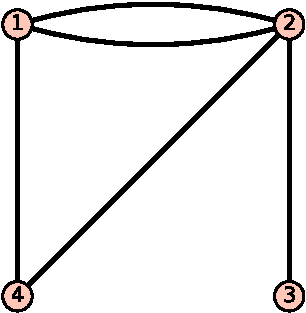
\includegraphics[scale=0.75]{u-crop}
        \end{figure}
        \vspace{-1em}
        {\large $U(G)$}
        \end{column}
        
        \begin{column}{0.5\textwidth}
        Volem computar $c_{\SUM}(3)$
        
        \vspace{1em}

        \begin{itemize}
            \item[] $\dist(3,1) = 2$ 
            \item[] $\dist(3,2) = 1$
            \item[] $\dist(3,4) = 2$ 
        \end{itemize}
        
        \vspace{1em}
        
        $\therefore c_{\SUM}(3) = 5$
        \end{column}
    \end{columns}
\end{frame}

\subsection{\texorpdfstring{$\MAX$}{MAX}}
\begin{frame}{Model $\MAX$}

Definim la funció de cost del model $\MAX$ com:

\begin{equation}
    c_{\MAX}(u) = \max \{ \dist(u, v) : v \in V(G) \} + (\kappa - 1)n^2
\end{equation}

On $\kappa$ és el nombre de components connexos de $U(G)$.

\vspace{2em}

El primer terme $\max \{ \dist(u, v) : v \in V(G) \}$ és l'excentricitat de $u$.

El terme $(\kappa - 1)n^2$ s'afegeix per incentivar decréixer el nombre de components connexos.

\end{frame}

\begin{frame}{Model $\MAX$}
    \begin{columns}
        \begin{column}{0.5\textwidth}
        \centering
        \begin{figure}
        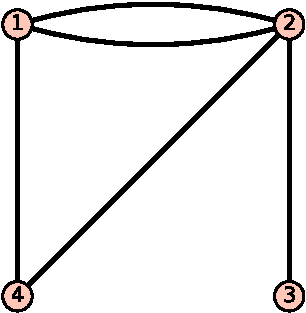
\includegraphics[scale=0.75]{u-crop}
        \end{figure}
        \vspace{-1em}
        {\large $U(G)$}
        \end{column}
        
        \begin{column}{0.5\textwidth}
        Volem computar $c_{\MAX}(3)$
        
        \vspace{1em}

        \begin{itemize}
            \item[] $\dist(3,1) = 2$ 
            \item[] $\dist(3,2) = 1$
            \item[] $\dist(3,4) = 2$ 
        \end{itemize}
        
        \vspace{1em}
        
        Cal tenir en compte que $\kappa = 1$
        
        \vspace{0.5em}
        
        \note{$n = 4$}
        
        $\therefore c_{\MAX}(3) = 2 + 0 \cdot 4^2 = 2$
        \end{column}
    \end{columns}
\end{frame}

\subsection{Resultats}
\begin{frame}{Resultats}
Es demostra que:

\begin{itemize}[<+->] 

    \note{A l'article s'estudien diverses propietats dels \emph{equilibrium graphs}. En particular s'analitza el diàmetre dels grafs en alguns casos especials. Aquest anàlisi resulta en uns límits del preu de l'anarquia (\emph{PoA}) pels diferents casos.}
    
    \item Per tota seqüencia no negativa $ (b_1, b_2, \dots , b_n)$ en el joc $ (b_1, b_2, \dots , b_n)\text{-BG} $ hi ha un equilibri de Nash i el preu d'estabilitat és $\Theta(1)$ en les dues versions.
    
    \vspace{1em}
    
    \item En els casos on la suma dels pressuposts és igual a $n-1$ el \emph{PoA}
    és~$\Theta(n)$ i~$\Theta(\log n)$ en~$\MAX$ i~$\SUM$ respectivament.
    
    \vspace{1em}
    
    \item El \emph{PoA} quan el pressupost de tots els jugadors és igual a $1$ és $\Theta(1)$ en les dues versions.
    
    \vspace{1em}
    
    \item A mesura que s'incrementa el pressupost dels jugadors el diàmetre del graf \textbf{no} disminueix. Per la versió de $\MAX$ hi han instàncies amb tots el pressuposts positius on el \emph{PoA} és $\Omega(\sqrt{\log n})$.
    
\end{itemize}
\end{frame}

\begin{frame}{Resultats}
\begin{itemize}[<+->] 
    
    \item En la versió $\SUM$ el \emph{PoA} té com a límit superior $2^{O(\sqrt{\log n})}$.

    \vspace{1em}
    
    \item Pel model $\SUM$, si cada jugador té pressupost $k$, llavors tots els \emph{equilibrium graphs} de diàmetre major $3$ seran $k$-\textsc{connected}.
    
\end{itemize} 

    \begin{figure}
    \centering
    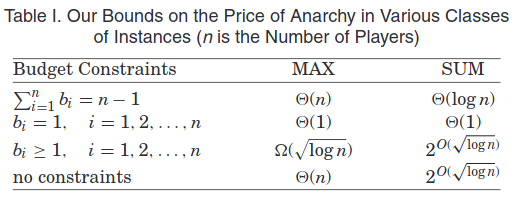
\includegraphics[width=0.7\textwidth]{Table1_PoA_Bounds}
    \caption{Taula extreta del article \cite{ehsani_bounded_2015}}
    \end{figure}
\end{frame}

\section{Best response és NP-hard}
\subsection{Theorem 2.1}
\begin{frame}{Teorema}

    L'article enuncia i demostra el següent teorema:
    
    \begin{theorem}
    The problem of finding a player's best response in both $\MAX$ and $\SUM$ versions of the bounded
    budget network creation games is NP-hard.
    \end{theorem}
    
    \vspace{2em}
    
    La demostració es basa en una reducció de \kcenter a $\MAX$ i de \kmedian a $\SUM$.
    On \kcenter i \kmedian són 
    NP-hard~\cite{hsu_easy_1979,lin_e-approximations_1992,megiddo_complexity_1984}.
    
\end{frame}

\note[itemize]{
\item A l’article enuncia i demostra el següent teorema
diu que el problema de trobar la best response tant en la version $\SUM$ com en la versió $\MAX$ del bounded budget network creation game es NP-hard.
\item La demostració que dona es basa en una reducció de 
\item \kcenter a la versió $\MAX$ i de 
\item \kmedian a la versió $\SUM$. 
\item On tant \kcenter com \kmedian son NP-hard.
}

% \begin{frame}{Articles citats}
% \begin{columns}

% \begin{column}{0.5\textwidth}
% \begin{figure}
% 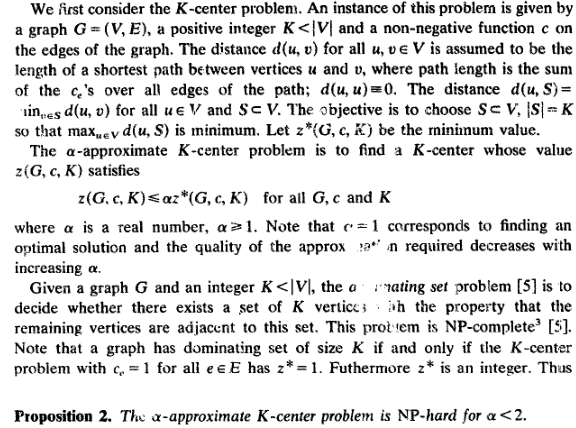
\includegraphics[width=\textwidth]{k-center_dominating_set}
% \caption{Wen-Lian Hsu i George L. Nemhauser. (1979) \cite{hsu_easy_1979} }
% \end{figure}

% \note[item] {
%     L'article de Wen-Lian \textbf{Hsu} i George L. \textbf{Nemhauser} es demostra que \kcenter es NP-hard fent una reduccio
%     de \emph{dominating set}.
%     \item L'article de \textbf{Lin i Vitter} al que fa referencia el nostre article original per referirse a la definicio
%     de \kmedian, citen al article de \textbf{Meggido i Supowit} en el que es demostren tant \kmedian com \kcenter
%     fent reduccions a 3-SAT.
% }
% \end{column}

% \begin{column}{0.5\textwidth}
% \begin{figure}
% 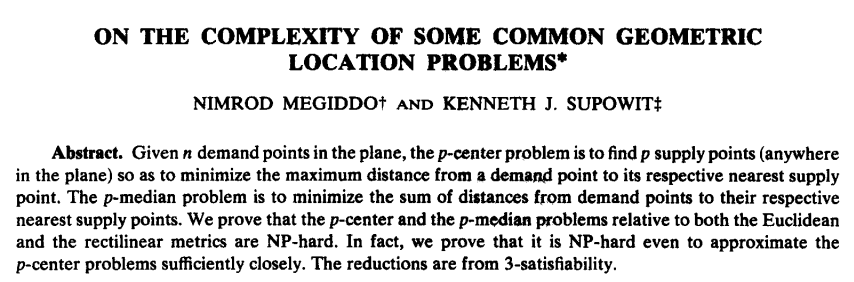
\includegraphics[width=\textwidth]{abstract_megiddo}
% \caption{Nimrod Megiddo i Kenneth Supowit. (1984) \cite{megiddo_complexity_1984} }
% \end{figure}
% \end{column}

% \end{columns}
% \end{frame}

\subsection{\kcenter}
\begin{frame}{\kcenter}

\begin{problem}[\kcenter]
Donat un graf no-dirigit $H$ i un enter positiu $k$ es vol trobar un subconjunt $S$ de $k$
vèrtexs que minimitzi la distància màxima de un vèrtex a $S$:

\begin{equation}
\min_{S \subseteq V(H):|S|=k} \left( \max_{v \in V(H)} \dist(v, S) \right)
\end{equation}
\end{problem}

\begin{equation}
    \dist(v, S) = \min \{ \dist(v, u) : u \in S \}
\end{equation}

\end{frame}
\note[itemize]{
\item El problema de \kcenter ens diu que donat un graf no dirigit $H$ i un enter positiu $k$,
es vol trobar un conjunt $S$ de $k$ vèrtex que minimitza la distancia màxima de un vèrtex a $S$:
\item Es pot expressar tal com es mostra.
\item La distància d'un vèrtex $v$ a $S$ és la distancia mínima de $v$ al vèrtex de $S$ mes proper 
}

\begin{frame}{\kcenter}
    \begin{figure}
    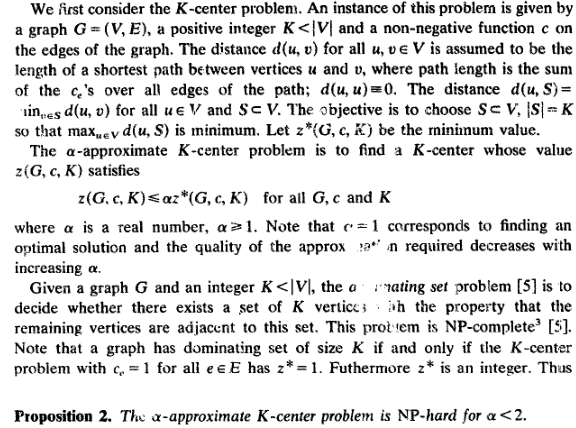
\includegraphics[width=0.5\textwidth]{k-center_dominating_set}
    \caption{Wen-Lian Hsu i George L. Nemhauser. (1979) \cite{hsu_easy_1979} }
    \end{figure}
\end{frame}
\note[itemize]{
    \item L'article cita un article de Hsu i Nemhauser en el cual es demostra que la 
    $\alpha$-aproximació de \kcenter és NP-hard per $\alpha<2$
    fent una reducció de dominating set (NP-complet).
    \item Un graf te un dominating set de mida $k$ iff el \kcenter amb cost 1 per tots els edges
    te com a millor resposta de tots els nodes un valor tal que la distancia és 1.
}

\subsection{Reducció de \kcenter a \texorpdfstring{$\MAX$}{MAX}}
\begin{frame}{Reducció de \kcenter a $\MAX$}
    Donat un graf no dirigit $H$ de $n$ vèrtexs i un enter positiu $k$ volem trobar una solució òptima a
    \kcenter.
    
    \vspace{2em}
    
    Considerem ara un graf $G$ tal que $U(G) = H$ i un joc $ (b_1, b_2, \dots , b_n, b_{n+1})\text{-BG} $ on
    $b_i$ és el grau de sortida del vèrtex $i$ de $G$ i $b_{n+1} = k$.
    
    \vspace{2em}
    
    La millor resposta (\emph{best response}) del jugador $n+1$ amb les estratègies de la resta marcades
    per $G$ és una solució òptima de \kcenter.
    
    \note{
        %TODO: explicar en detall aixo
        
        La distancia de qualsevol vèrtex a $n+1$ serà sempre 1 + la distancia a la solució de \kcenter (conjunt $S$)
    }
\end{frame}
\note[itemize]{
\item Per fer la reducció de \kcenter a $\MAX$ tenim que donat un graf no dirigit $H$ amb $n$ vertex i un enter positiu $k$
volem trobar una solució optima a \kcenter.

\item Si considerem ara un graf $G$ tal que $U(G) = H$ i un joc BG on $b_i$ es el grau de sortida del vertex $i$-essim de
$G$ i $b_{n+1} = k$

\item tenim que la millor resposta del jugador $n+1$ amb les estratègies fixades per $G$ per la resta de jugadors 
es una solució òptima de \kcenter.

\item Aixo ho podem veure si ens adonem que la estratègia de $b_{n+1}$ el que fa es seleccionar $k$
vèrtex del graf tal que la distancia màxima a la resta dels vèrtex del graf es mínima. I com que el vèrtex $n+1$ 
esta sempre a distancia 1 del vèrtex  de la seva estratègia $S$, la distancia de qualsevol vèrtex a $S$ serà
igual a la distancia al vèrtex $n+1$ - 1 i per tant estem minimitzant la distancia màxima al conjunt $S$.
}

\subsection{\kmedian}
\begin{frame}{\kmedian}

\begin{problem}[\kmedian]
Donat un graf no dirigit $H$ i un enter positiu $k$ es vol trobar un conjunt $S \subseteq V(H)$ de $k$ vèrtexs
tal que es minimitzi la suma de les distancies de cada vèrtex en $V(H)$ a el vèrtex més proper
de $S$.

\begin{equation}
\min_{S \subseteq V(H):|S|=k} \left(
    \sum _{v \in V(G)} \dist(v, m_S(v))
\right)
\end{equation}

On $m_S(v)$ és el vèrtex de $S$ més proper a $v$.
% quizas aqui podemos poner algo en plan m_S(v) = min_{u \in S} dist(u,v)

\end{problem}

\end{frame}
\note[itemize]{
\item El problema de \kmedian ens diu que donat un graf no dirigit $H$ 
i un enter positiu $k$ es vol trobar un subconjunt $S$ de $V(H)$ de $k$ vèrtex tal que es minimitzi 
la suma de les distancies de cada vèrtex de $V(H)$ al vèrtex mes proper de $S$.
\item Es pot expressar formalment aixi:
\item on $m_S(v)$ es el vèrtex de $S$ mes proper a $v$.
\item (també es podria haver expressat com a \kcenter utilitzant la definició de distancia de vèrtex a conjunt de vèrtex).
}

\begin{frame}{\kmedian}
\begin{columns}

\begin{column}{.5\textwidth}
    \begin{figure}
    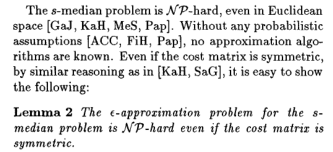
\includegraphics[width=\textwidth]{k-median_ref}
    \caption{Jyh-Han Lin i Jeffrey Scott Vitter. (1992) \cite{lin_e-approximations_1992}} 
    \end{figure}
\end{column}

\begin{column}{.5\textwidth}
    \begin{figure}
    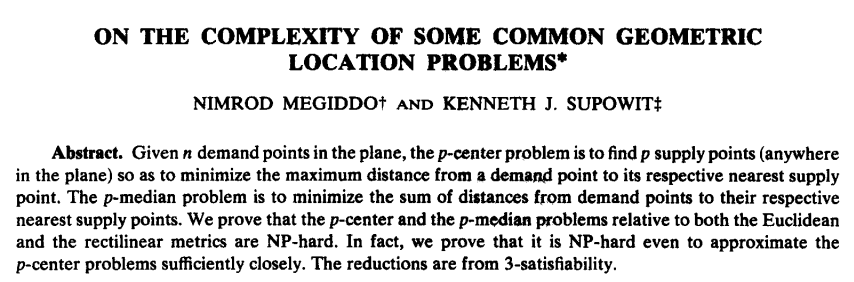
\includegraphics[width=\textwidth]{abstract_megiddo}
    \caption{Nimrod Megiddo i Kenneth Supowit. (1984) \cite{megiddo_complexity_1984} }
    \end{figure}
\end{column}

\end{columns}
\end{frame}
\note[itemize]{
     \item L'article de \textbf{Lin i Vitter} al que fa referencia el nostre article original per referir-se a la definició
     de \kmedian, citen (entre altres) l'article de \textbf{Meggido i Supowit} en el que es demostren
     tant \kmedian com \kcenter fent reduccions des de 3-SAT.
}

\subsection{Reducció de \kmedian a \texorpdfstring{$\SUM$}{SUM}}
\begin{frame}{Reducció de \kmedian a $\SUM$}

Apliquem el mateix principi que en el cas de \kcenter i $\MAX$:

    \vspace{2em}

    Donat un graf no dirigit $H$ de $n$ vèrtexs i un enter positiu $k$ volem trobar una solució òptima a
    \kmedian.
    
    \vspace{2em}
    
    Considerem ara un graf $G$ tal que $U(G) = H$ i un joc $ (b_1, b_2, \dots , b_n, b_{n+1})\text{-BG} $ on
    $b_i$ és el grau de sortida del vèrtex $i$ de $G$ i $b_{n+1} = k$.
    
    \vspace{2em}
    
    La millor resposta (\emph{best response}) del jugador $n+1$ amb les estratègies de la resta marcades
    per $G$ és una solució òptima de \kmedian.
    
\end{frame}
\note[itemize]{
\item Apliquem el mateix mètode que en el cas de \kcenter i $\MAX$:
\item Tenim un graf no dirigit $H$ de $n$ vèrtex amb un enter positiu $k$ on volem trobar una solució optima a \kmedian.

\item Si considerem un graf $G$ tal que $U(G) = H$ i un joc BG on 
$b_i$ es el grau de sortida del vèrtex $i$-essim de $G$ i $b_{n+1} = k$
tenim que la millor resposta del jugador $n+1$ es una solució optima de \kmedian.
\item Al igual que amb \kcenter la millor resposta del jugador $n+1$ el que farà es seleccionar 
els $k$ vèrtex tal que es minimitzi la suma de la resta de vèrtex a $n+1$
(i com que la distancia es la mateixa + 1 es també la distancia que minimitza la 
suma al conjunt de vèrtex que es el que es busca a \kmedian )
\item La distancia de qualsevol vèrtex a $n+1$ serà sempre 1 + la distancia a la solució de \kmedian (conjunt $S$)
\item La suma es nomes dels elements mes propers, per tant es manté la condició de $\dist$ a $m_S(v)$
\item Aixi doncs tant la versió $\SUM$ com la $\MAX$ son NP-hard.
}


\begin{frame}{Bibliografia}
\printbibliography
\end{frame}

\begin{frame}{Index}
  \tableofcontents
\end{frame}

\begin{frame}
\end{frame}


\end{document}

